\documentclass[12pt]{article}
%%% ========== Package setup ==========
\usepackage{listings}   % Script listing package
\usepackage{wrapfig}    % Wrap Figure or table package
\usepackage{multicol}   % Multicolumn package
\usepackage{pdfpages}   % Include pdf files

%%% ========== Format setup ==========
%% Setup chinese words encoder
\usepackage{xeCJK}
\XeTeXlinebreaklocale "zh"
\XeTeXlinebreakskip = 0pt plus 1pt

%% More word fonts
\usepackage{fontspec}
\setmainfont{Times New Roman}
\renewcommand{\familydefault}{\rmdefault}
\setCJKmainfont{標楷體}

%% Chinese paragraph format
\usepackage{indentfirst}
\setlength{\parindent}{2em}

%% Page margin
\usepackage[a4paper, total={6in,8in}]{geometry}

%%% ========== Document ==========
\begin{document}
\newcommand{\MakeTitlePage}[1]{
\begin{titlepage}
    \begin{center}

        \fontsize{50}{10}
        \selectfont
        Optimal Control

        \vspace{1cm}

        \fontsize{30}{10}
        \selectfont
        Final exam

        \vspace{11cm}

        \begin{tabular}{ r l }
            班級: & 航太四A \\ [10pt]
            姓名: & 吳柏勳 \\ [10pt]
            學號: & 407430635 \\ [10pt]
            座號: & 3 \\ [10pt]
        \end{tabular}

    \end{center}
\end{titlepage}
}
\MakeTitlePage{}
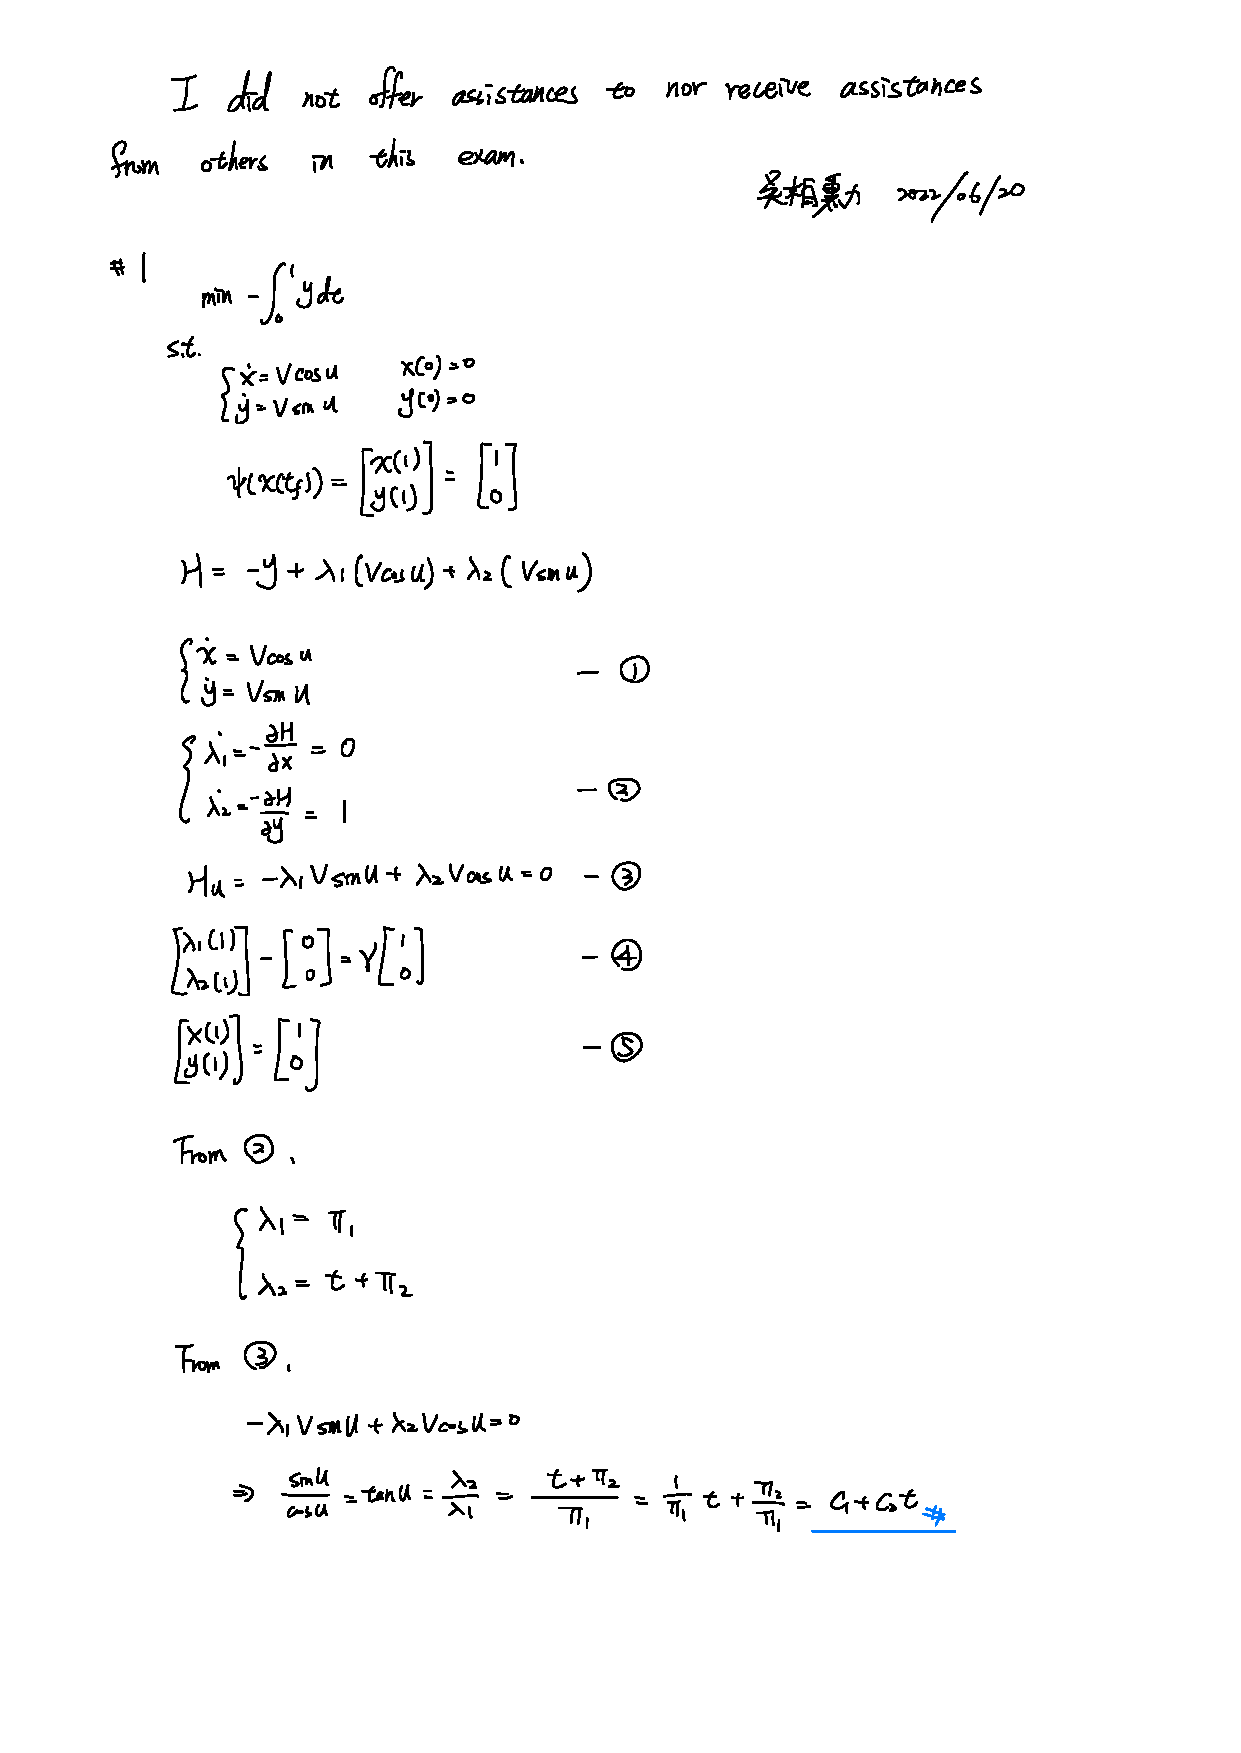
\includepdf[pages=-]{handout.pdf}

\subsection*{\#4(b)}

\begin{verbatim}
clear;clc;close all
% System parameter
A = [-0.2640   0.7203   0      -9.8063
     -1.4406  -8.0534  10.5360  0
      0.7936 -10.4977 -20.2975  0
      0        1        0       0     ];
B = [ 0       2.8510
     -0.1392  0
     -2.4104  0
      0       0     ];
C = [0 0 1 0];
D = zeros(1,2);

% Constrain parameter
yd = 1;
psi = [0 0 1 0]';
Mf = diag([1 1 1 1]).*factor;

% Tune parameter
factor = 1;
Qd = 100.*factor;               % weight of tracking
Rd = diag([100 100]).*factor;   % weight of control
Qf = diag([1 1 1 1]).*factor;   % weight of terminal error

Q = C'*Qd*C;
N = C'*Qd*D;
R = Rd + D'*Qd*D;

% Terminal condition
x_tf = psi;
s_tf = Mf'*Qf*Mf;
s_tf = reshape(s_tf, [16,1]);
g_tf = -Mf'*Qd*psi;
state_tf = [x_tf; s_tf; g_tf];

LQT = @(t, state) NC(t, state, A, B, C, D, Q, R, N, Qd, yd);
[t, state] = ode45(LQT, [5 0], state_tf);

% Plot of result
figure()
plot(t, state(:,1))
xlabel("t"); ylabel("u")
grid on

figure()
plot(t, state(:,2))
xlabel("t"); ylabel("w")
grid on

figure()
plot(t, state(:,3))
xlabel("t"); ylabel("p")
grid on

figure()
plot(t, state(:,4))
xlabel("t"); ylabel("\theta")
grid on
\end{verbatim}

\subsection*{\#4(c)}
\large
No, it can't be solved by this method. It may figure out an answer but the solution is out of sense because the initial state we figure out approaches to the infinity. And it is difficult to solve this problem by tuning the parameters.

\newpage
\begin{multicols*}{2}
    \centering
    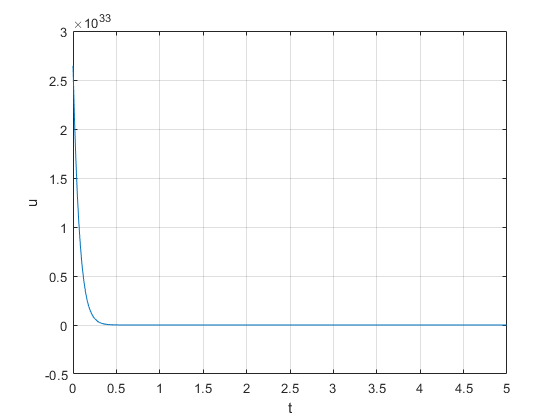
\includegraphics [width=3in]{Final_01.png}
    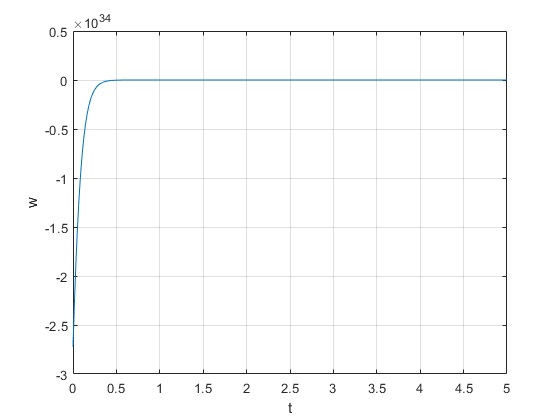
\includegraphics [width=3in]{Final_02.png}
    \vfill
    \columnbreak

    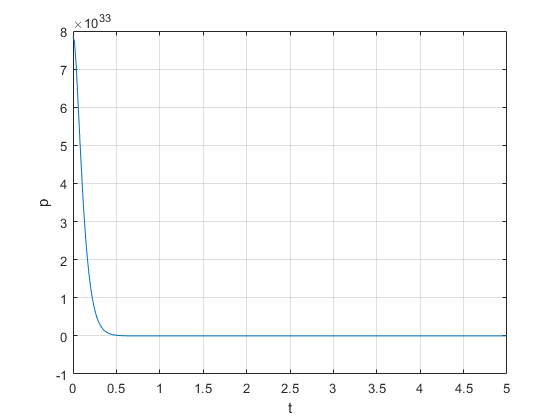
\includegraphics [width=3in]{Final_03.png}
    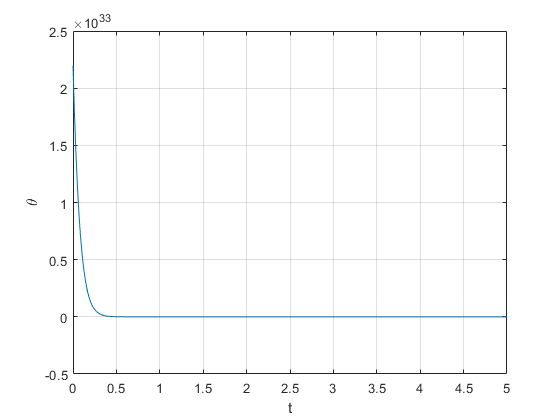
\includegraphics [width=3in]{Final_04.png}

\end{multicols*}

\subsection*{function of necessary condition}

\begin{verbatim}
function dstate = NC(t, state, A, B, C, D, Q, R, N, Qd, yd)
    % state define: [x(1:4), s(5:20), g(21:24)]'

    x = state(1:4);
    s = reshape(state(5:20), [4,4]);
    g = state(21:24);
    lambda = s*x + g;
    u = inv(R)*(-N'*x-B'*lambda);

    inv_R = inv(R);

    dx = A*x + B*u;
    ds = -s*(A-B*inv_R*N') - (A-B*inv_R*N')'* - Q ...
         + N*inv_R*N' + s*B*inv_R*B'*s;
    dg = (-(A-B*inv_R*N')' + s*B*inv_R*B')*g + C'*Qd*yd;

    dstate = zeros(24,1);
    dstate(1:4) = dx;
    dstate(5:20) = reshape(ds, [16,1]);
    dstate(21:24) = dg;

end
\end{verbatim}

\end{document}

